\subsubsection*{Zadanie~9.15.}
Tak, taki ostrosłup istnieje. Aby go skonstruować, możemy na przykład rozważyć w~podstawie trapez równoramienny, w~którym proste zawierające ramiona \(BC\) i~\(DA\) są do siebie prostopadłe:
\begin{mathfigure*}
    \coordinate (A) at (-4, 0);
    \coordinate (B) at (4, 0);
    \coordinate (C) at (2, 2);
    \coordinate (D) at (-2, 2);
    \coordinate (X) at (0, 4);
    \drawrightangle{A--X--B};
    \draw (A) -- (B) -- (C) -- (D) -- cycle;
    \draw[dotted] (X) -- (C);
    \draw[dotted] (X) -- (D);
    \fillpoint*{A}[\(A\)][below left];
    \fillpoint*{B}[\(B\)][below right];
    \fillpoint*{C}[\(C\)][above right];
    \fillpoint*{D}[\(D\)][above left];
    \fillpoint*{X}[\(X\)][above];
\end{mathfigure*}
\noindent
Punkt \(X\) to przecięcie tych dwóch prostych. Teraz, jeśli podniesiemy punkt \(X\) nad płaszczyznę, to uzyskamy \(Y\). Ściany \(CBY\) i~\(DAY\) będą prostopadłe do podstawy, ponieważ zawierające je płaszczyzny \(XBY\) i~\(XAY\) są do niej prostopadłe. Będą również prostopadłe między sobą, ponieważ kąt \(\angle{BXA}\) jest prosty.
\begin{figure}[H]
    \centering
    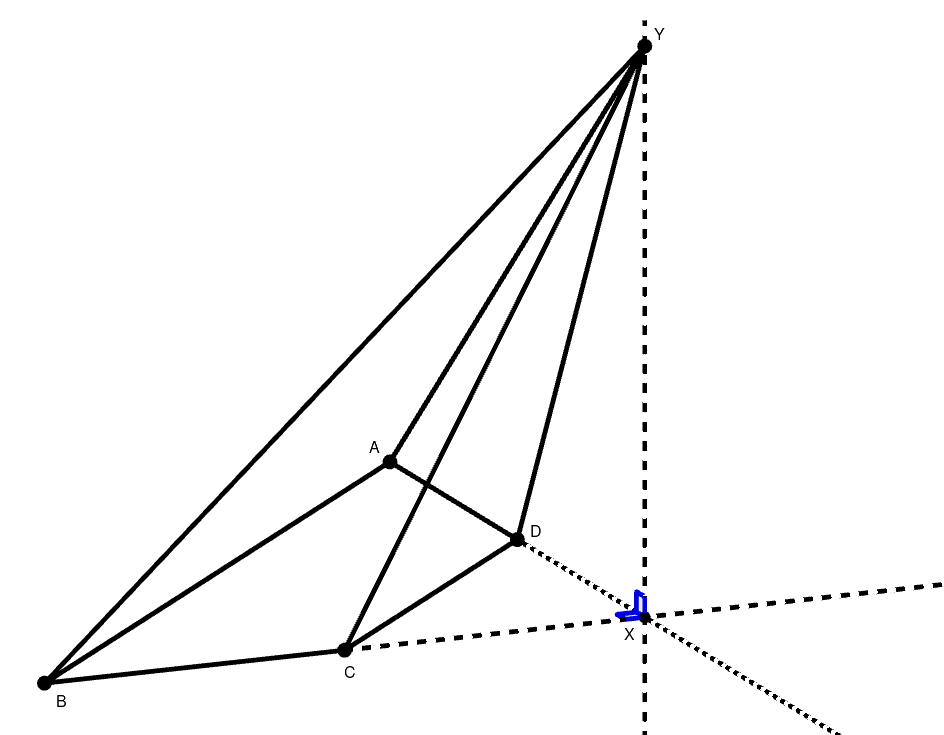
\includegraphics[width=\textwidth]{img/2021_02_12/15/space.png}
\end{figure}
\noindent
Taki ostrosłup spełnia więc warunki zadania.
\newpage
\subsubsection*{Zadanie~9.16.}
Ponieważ wszystkie krawędzie boczne mają równe długości, to spodek wysokości na podstawę jest środkiem okręgu opisanego na podstawie.
\begin{figure}[H]
    \centering
    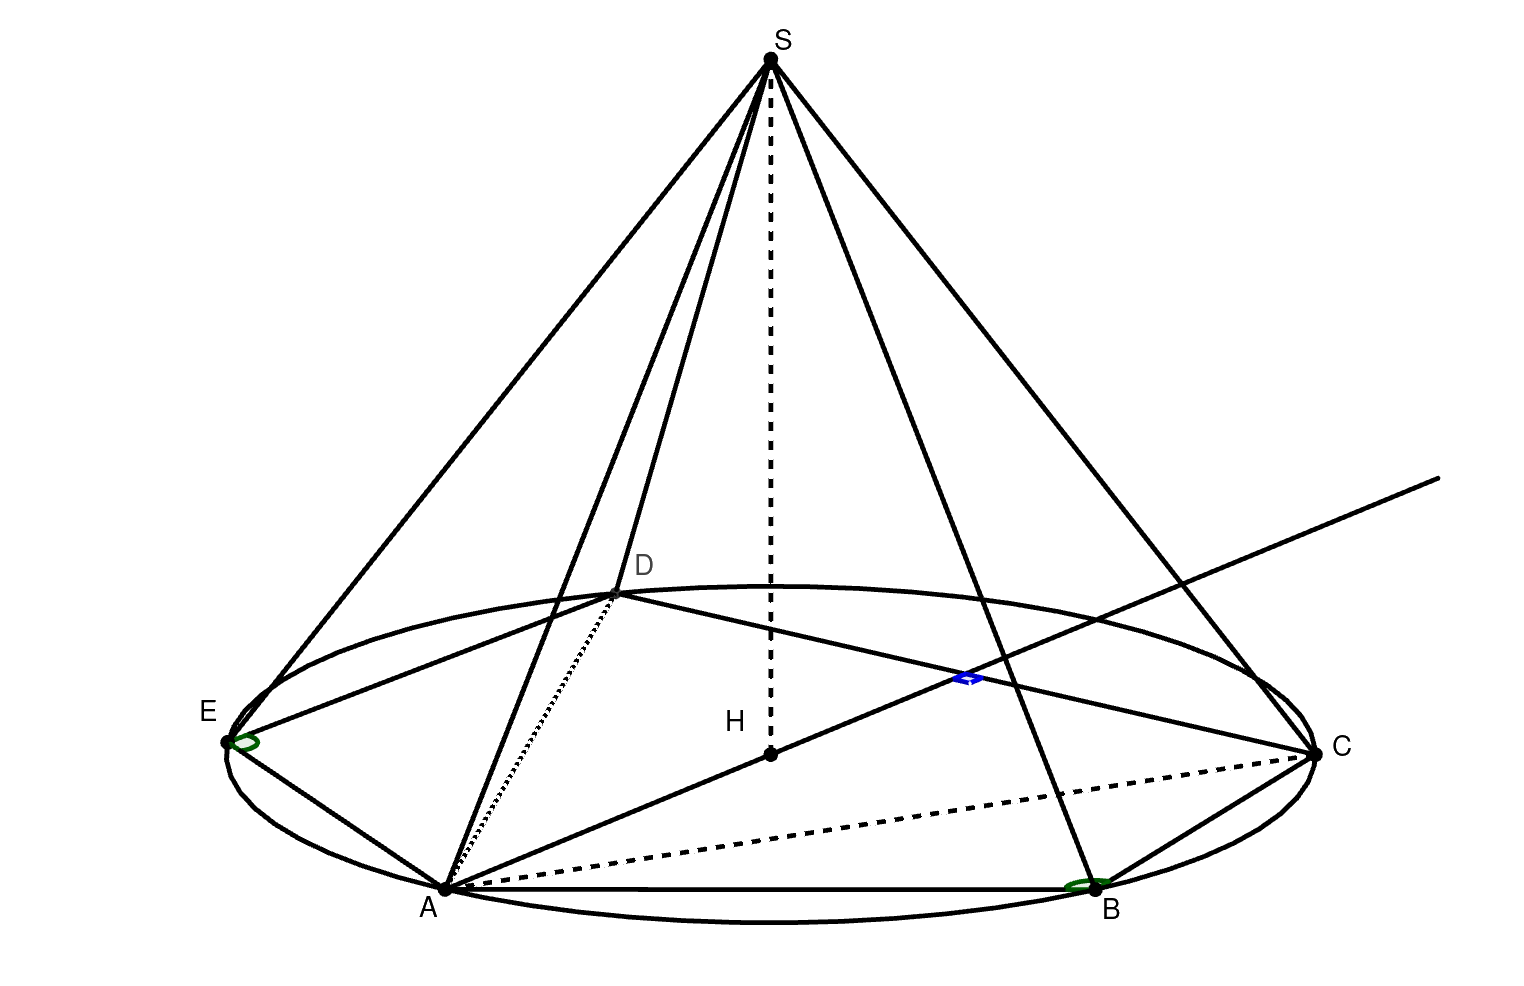
\includegraphics[width=\textwidth]{img/2021_02_12/16/space.png}
\end{figure}
\noindent
Ponieważ kąty \(\angle{ABC}\) i~\(\angle{AED}\) wpisane w~ten okrąg mają równe miary, to łuki, na których są oparte, muszą mieć równe długości, czyli cięciwy odcinające te łuki także muszą być równej długości. Zatem \(CA = DA\), czyli \(\triangle{CAD}\) jest równoramienny. W~trójkącie równoramiennym środek okręgu opisanego leży na wysokości opuszczonej z~wierzchołka wspólnego dla obydwu ramion, ponieważ jest ona jednocześnie symetralną podstawy. Zatem \(AH \perp CD\). Natomiast prosta \(AH\) jest rzutem prostej \(AS\) na płaszczyznę podstawy, więc z~twierdzenia o~trzech prostych prostopadłych mamy
\begin{equation*}
    AS \perp CD
\end{equation*}
\qed

